\section{Introduction}
\label{sec:intro}

% Fig. 1 -- teaser (figure*, top of page 1 or 2)
\begin{figure*}[tbp]
  \centering
  \subcaptionbox{Where exact repeats live (potential tier)\label{fig:scope}}{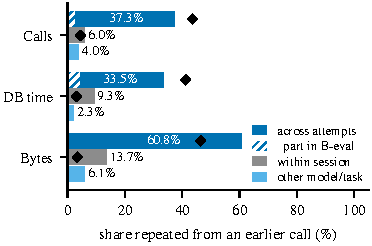
\includegraphics[height=1.62in]{figures/fig1a_scope}}\hfill
  \subcaptionbox{Reuse grows with $N$ (potential tier)\label{fig:ncurve}}{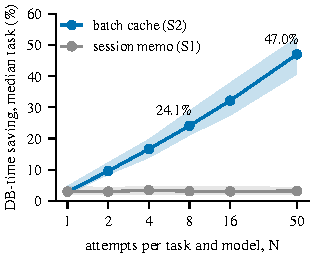
\includegraphics[height=1.62in]{figures/fig1b_ncurve}}\hfill
  \subcaptionbox{What each admission tier admits\label{fig:tiers}}{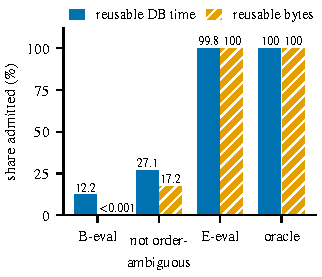
\includegraphics[height=1.62in]{figures/fig1c_tiers}}
  \caption{Where the database work of repeated agent runs repeats, and how much of it each admission tier can reuse
  on DAB. (a) Shares of calls, isolated DB-execution time and payload
  bytes among the 70,173 oracle-admitted calls, by the scope of the earlier exact repeat. The scopes are another
  attempt of the same task and model, the same session, and another model's or task's runs. Shares are pooled over 200
  random attempt orders. Diamonds mark the median task, and hatching marks the part in the B-eval subset. (b)
  Median-task saving of isolated DB-execution time in an unbounded, oracle-gated simulation with 200 resamples. S1 is
  a per-session cache, and S2 is a cache shared by a batch of $N$ attempts of one model on one task. Bands show the
  task-bootstrap 95\% CI, and $N=50$ uses the 268 of 270 task--model cells with 50 runs. (c) Share of the
  cross-attempt reusable DB time and bytes in the B-eval (certified), E-eval (assumption-based) and oracle (potential)
  subsets. The bar ``not order-ambiguous'' covers all calls except the successful ones with at least two distinct rows
  and no top-level \texttt{ORDER BY}. It is a conservative upper bound for any rule that guarantees serialized bytes across query plans in engine row order.}
  \label{fig:teaser}
  \Description{Three panels. Left: horizontal bars showing that repeats across attempts carry 37.3, 33.5 and 60.8 percent of calls, DB time and bytes, against 6.0, 9.3 and 13.7 percent within a session. Middle: lines showing the batch cache saving rising from 3 to 47 percent of DB time as attempts grow from 1 to 50 while the session cache stays near 3 percent. Right: bars showing the B-eval subset holds 12.2 percent of reusable DB time and almost no bytes, the calls that are not order-ambiguous 27.1 percent of the time and 17.2 percent of the bytes, while the E-eval subset and the oracle admit nearly all.}
\end{figure*}


LLM data agents are rarely run once on a task. A deployment retries a failed attempt or samples several attempts and
keeps the most consistent answer \cite{wang2023selfconsistency,brown2024monkeys}. It also evaluates an agent with $k$
trials per task and serves many users who ask the same question of the same data. Every attempt queries the same
database snapshot again. A cache inside one agent session cannot see that another attempt already ran the same query.
A data agent answers an analytical question by letting an LLM plan and issue database queries through a tool. It then
reads the results and post-processes them in Python \cite{ma2026dab,yao2023react}. The DAB benchmark runs each of its
54 multi-database tasks about 50 times with each of five LLMs against one dataset snapshot \cite{ma2026dab}. One DAB
run issues 5.7 database calls on average, and the 13,482 released runs issue 76,213.

For a data system, this repetition is both an opportunity and a cost. The database time of an attempt is
heavy-tailed. The median attempt spends 28.5\,ms executing its successfully replayed calls in isolation, and the
95th-percentile attempt spends 14.4\,s. A single result reaches 771\,MB when written to a file for the agent's Python
code. Recent work frames agents as a first-class data-system workload. The CIDR'26 vision of agent-first data systems
argues that agents speculate redundantly across attempts \cite{liu2026overlords}. TVCACHE caches tool results across
the parallel rollouts of LLM post-training \cite{kumar2026tvcache}. Reuse for the database calls of agent runs that
span several models and engines raises three open questions. Figure~\ref{fig:teaser} previews the results that answer them.

\begin{itemize}
  \item \textbf{Q1: Locality.} Where does the work repeat: within a session, across attempts of a task, or across
  models and tasks? The answer weights repeats by execution cost and result bytes, not only by call count.
  \item \textbf{Q2: Admissibility.} What can be reused while the agent sees byte-identical results? An exact reuse
  reproduces what a completed call shows the agent: the tool message, the bound value and any result file.
  \item \textbf{Q3: Ownership.} Who owns a reused result? At the tool boundary a result has two consumers. The LLM reads a preview, and the agent's Python code reads a file. Its owner decides what it costs to store and whether
  one attempt can corrupt it for another.
\end{itemize}

We answer these questions with a replay-based study of the public DAB release. We re-execute the 41,616 distinct
database--query pairs of the 13,482 runs in isolation, up to three times each, in a version-pinned runtime. The replay
uses the benchmark's own execution and serialization path. It attaches an execution cost, a result size and a
fidelity record to every replayed call. We attribute each call to the innermost scope in which an exact-text
equivalent occurred earlier. We resample $N$ attempts per task and model to measure how reuse grows with $N$. We
separate three admission tiers: what a static certificate admits, what a pinned runtime reproduces, and what an oracle
could reuse. We then compare six reuse designs at the tool boundary with an exact-accounting simulator and with live
runs. The live runs return the harness's exact tool messages and files and execute the agents' own Python consumers.

\textbf{F1: Cross-attempt locality.} We consider the calls whose replay is equivalent to the recorded observation. Exact repeats from other attempts of the same task and model carry 33.5\% of the isolated DB-execution time and 60.8\% of the result bytes. Repeats within the same session carry 9.3\% and 13.7\%. Per task the contrast is sharper, with medians of
41.2\% against 3.2\% and a larger cross-attempt median in all 12 datasets. In an unbounded simulation, a cache shared by a batch saves 24.1\% of the median task's oracle-admitted DB time at eight attempts. It
saves 47.0\% at fifty attempts, while a per-session cache stays near 3\% at every $N$. Four public leaderboard
harnesses that run DAB's tasks with other agent designs show the same ordering.

\textbf{F2: Certifiability--payoff divergence.} The cross-attempt payoff is recovered by runtime qualification rather
than by static certification. A conservative static certificate of byte stability admits 7.5\% of all calls and
0.023\% of the payload bytes. Of the cross-attempt reusable work it admits 12.2\% of the DB time and 0.00005\% of the
bytes. No sharper rule with the same across-plan guarantee closes the gap. The reason is that 58.7\% of the successful calls return at least two distinct rows without a top-level \texttt{ORDER BY}. A pinned runtime that we qualified offline
recovers the payoff in this workload. Every statically admissible DAB call whose replay succeeded was byte-stable. So
was every statically admissible query from four additional harnesses whose replay succeeded. Byte stability of these
calls is thus an empirical property of the qualified runtime.

\textbf{F3: Ownership governs storage cost.} This exploratory study uses the calls that the offline-qualified pinned runtime reproduces. At eight attempts, a simulated private-copy cache writes 1.70$\times$ the no-sharing bytes for the median task. A read-only shared
store with one alias per attempt writes 0.448$\times$ the bytes of private copies for the median task with spilled
results. It keeps 0.76$\times$ the peak footprint of no sharing when every attempt's outputs are retained. On the 12
calibration cells, live bytes written and footprint match the simulator in all 480 runs. The shared store reaches the
footprint of copy-on-write clones without reflink support and refuses the agents' writes. A live tool-boundary replay
covers one eight-attempt batch from each of the 270 task--model cells, 11,309 calls in all. Among its 2,443 cached hits, no cached value differed where both designs returned a result. Two hits returned a result where the uncached execution failed under load. All 4,655 consumer executions whose two uncached runs agreed produced the same output under reuse. Reference pinning keeps aliases valid under concurrent attempts.

This paper makes four contributions. The first is a replay-based methodology for the database work of repeated agent runs (Section~\ref{sec:method}). It yields a cost and fidelity table for 41,616 distinct agent queries and three admission tiers. The second is a characterization of where that work repeats and how reuse grows with the
number of attempts (Section~\ref{sec:locality}). The third is a measurement of how much reusable work each admission
tier admits (Section~\ref{sec:certify}). The fourth is a case study of result ownership at the tool boundary
(Section~\ref{sec:ownership}). Section~\ref{sec:boundaries} delimits the scope and derives design implications.
